\documentclass[11pt]{article}
\usepackage[a4paper,margin=25mm]{geometry}
\usepackage{amsmath,amssymb,amsthm,mathtools,booktabs,array,xcolor,tikz}
\usepackage[T1]{fontenc}\usepackage{lmodern}
\usepackage[colorlinks=true,linkcolor=teal,citecolor=teal,urlcolor=teal]{hyperref}
\hypersetup{pdftitle={Moment-Compatible Readouts and Exceptional Pullbacks},pdfauthor={Akari Hayami (Jian-Yu Huang)},pdfsubject={Local continuation 0.04}}
\newtheorem{theorem}{Theorem}[section]
\newtheorem{proposition}[theorem]{Proposition}
\newtheorem{lemma}[theorem]{Lemma}
\newtheorem{corollary}[theorem]{Corollary}
\theoremstyle{definition}\newtheorem{definition}[theorem]{Definition}
\theoremstyle{remark}\newtheorem{remark}[theorem]{Remark}
\newcommand{\R}{\mathbb R}\newcommand{\C}{\mathbb C}\newcommand{\Z}{\mathbb Z}
\newcommand{\Q}{\mathbb Q}
\newcommand{\Hom}{\operatorname{Hom}}\newcommand{\RHom}{\operatorname{RHom}}
\newcommand{\End}{\operatorname{End}}\newcommand{\inte}{\operatorname{int}}
\newcommand{\orr}{\mathrm{or}}
\title{Moment-Compatible Readouts and Exceptional Pullbacks\\
for the Bicomplex Signal Surface}
\author{Akari Hayami (Jian-Yu Huang)}
\date{2 October 2026\\\small Research continuation 0.04; local working draft}
\begin{document}\maketitle
\begin{abstract}
Early drafts asserted that a power constraint and the moment assignment
$(|z_1|^2,|z_2|^2)=(\cos t,1-\cos t)$, followed by a ``geometric projection''
$\R^4\to\R^3$, produce the ruled signal surface. We prove that no readout which
is real-analytic along the circle $z_1=0$ realizes the surface under that
assignment, whatever state family is used. This excludes affine projections,
every real polynomial readout and every polynomial in a bicomplex variable and
its conjugates. The obstruction is sharp. An explicit continuous state family
and an explicit $C^\infty$ readout do realize the surface, and on either half of
the source a real-analytic readout exists although no affine one does. Phase-invariant and
mixed-state readouts fail without any regularity assumption. We also show that
the exceptional pullback of every continuous map from a convex parameter domain to the
plane is the extension by zero of the constant sheaf on its interior. The draft
formula $i^*\Psi^!\Z\simeq\Z[-1]$ on the fold locus therefore holds at no
point, and $\Psi^!\Z$ cannot detect folds. The fold is detected instead by
failure of the comparison map required for cohomological smoothness. Finally,
the log-scale versus linear-scale decorrelation gap is a ratio of normalizing
window masses and involves no arithmetic.
\end{abstract}

\section{Sources and scope}\label{sec:scope}
Three historical records are kept distinct; their SHA-256 values are
\begin{center}\footnotesize
\begin{tabular}{@{}ll@{}}
v12 PDF, 43 pp.\ (authority) & \texttt{4ebb8f0a7d6e88a6c5cd97f65d224b4e938867cabad54f057d3ceafb24167d5a}\\
v7 PDF, 26 pp. & \texttt{6cefa5258257f3a23e35b5dd5cbe123b7af0ed3319c3a614b1c8d54c94bd654f}\\
ancestor TeX & \texttt{4c0a5b5a8287ab5559c892b2ee21c170984e5f9649481018f851095118a1f016}
\end{tabular}
\end{center}
The ancestor TeX has 1,908 lines.
The v7 draft, dated July 2026 on its title page, is registered here as a
non-authoritative historical draft. It is neither v12 nor a demonstrated
product of the ancestor TeX. Equal numbering does not imply equal content.
Page numbers below are physical pages of the cited PDF.

All three records contain the moment assignment of \S\ref{sec:moment}: v7
\S3 and Definition~3.1 on p.~2, the ancestor \S3, and v12 \S3 and
Definition~3.1 on p.~4. The exceptional-pullback,
monodromy-endomorphism and log-window statements of
\S\S\ref{sec:shriek}--\ref{sec:windows} are v7 Proposition~8.3 and
Remarks~8.4 and 8.16 (pp.~10--11, 18), Definition~8.9 to Corollary~8.11
(pp.~14--15) and Proposition~8.13 with Remark~8.14 (pp.~15--17). The ancestor
and v12 no longer assert the exceptional-pullback identity; they do not decide
it either. The results below are new constructions, proofs and counterexamples.
They are not recoveries of missing historical derivations.

Throughout,
\[
 S(t,u)=\bigl(c+2u(1-c),(1-u)s,uQ\bigr),\qquad
 c=\cos t,\ s=\sin t,\ Q=\sqrt{c(2-c)},
\]
on $D=[-\pi/2,\pi/2]\times[0,1]$. Put $D_\circ=(-\pi/2,\pi/2)\times[0,1]$ and
$D_+=[0,\pi/2]\times[0,1]$. The edges and the polar ruling map to
\begin{equation}\label{eq:edges}
 S(\pm\tfrac\pi2,u)=(2u,\pm(1-u),0),\qquad S(0,u)=(1,0,u).
\end{equation}
The two edge segments lie on distinct lines through the apex $(2,0,0)$. The
ruling line $\{(1,0,z)\}$ is skew to both edge lines.

\section{The ancestral moment assignment}\label{sec:moment}
Let $S^3=\{z\in\C^2:|z_1|^2+|z_2|^2=1\}$, and let
$C_0=\{(0,w):|w|=1\}$ and $C_1=\{(w,0):|w|=1\}$. The bicomplex idempotent
coordinates identify the algebra with $\C\oplus\C$; we write the two components
as $z_1,z_2$. A real polynomial in a bicomplex variable and its three standard
conjugates is a real polynomial in $\Re z_j,\Im z_j$.

\begin{definition}\label{def:moment}
Let $D'\subset D$. A \emph{moment-compatible state family} on $D'$ is any map
$z:D'\to S^3$ with $|z_1(t,u)|^2=\cos t$. No continuity is assumed. A
\emph{readout} is a map $P:U\to\R^3$ on a set $U\subset\C^2$ containing $z(D')$;
it \emph{realizes} $S$ if $P\circ z=S$ on $D'$. It is \emph{real-analytic along
$C_0$} if $C_0\subset U$ and $\beta\mapsto P(0,e^{i\beta})$ is real-analytic.
\end{definition}

Every state with $t=\pm\pi/2$ lies on $C_0$, and every state with $t=0$ lies on
$C_1$. This alone already excludes the gauge-invariant readouts.

\begin{proposition}[Phase-invariant and mixed-state readouts]\label{prop:gauge}
Suppose $D'$ contains two points $(\pi/2,u_1)\neq(\pi/2,u_2)$, or two such
points at $t=-\pi/2$. No readout with $P(e^{i\gamma}z)=P(z)$ realizes $S$ on $D'$.
In particular no function of the density matrix $zz^*$ does, including all
Hermitian expectation values. If density matrices $\rho(t,u)\geq0$ of trace one
with $\rho_{11}=\cos t$ replace pure states, no function of $\rho$ realizes $S$.
\end{proposition}
\begin{proof}
$C_0$ is a single orbit of the global phase, so such a readout is constant on
$C_0$. By \eqref{eq:edges}, however, $S$ takes distinct values at the two edge
points. For mixed states, $\rho_{11}=0$ and positivity force $\rho_{12}=0$, so
$\rho=\mathrm{diag}(0,1)$ at both points.
\end{proof}

\begin{lemma}[Analytic curves and lines]\label{lem:analytic}
Let $p:J\to\R^3$ be real-analytic on an open interval $J$ or on the circle. For
every line $\ell$, either $p(J)\subset\ell$ or $p(J)\cap\ell$ is countable.
Hence $p(J)$ cannot contain uncountable subsets of two distinct lines.
\end{lemma}
\begin{proof}
Choose $x_0\in\ell$ and unit normals $n_1,n_2$ to $\ell$. If $p(J)\not\subset\ell$,
some $f_k=n_k\cdot(p-x_0)$ is a nonzero real-analytic function, so its zero set is
discrete in $J$ and hence countable. It contains $p^{-1}(\ell)$. If $p(J)$
met two distinct lines in uncountable sets, it would lie in both lines. Their
intersection has at most one point, a contradiction.
\end{proof}

\begin{theorem}[Analytic rigidity]\label{thm:rigidity}
Let $z$ be a moment-compatible state family and $P$ a readout that realizes $S$
on $D'$.
\begin{enumerate}
\item If $D'=D$, then $P$ is not real-analytic along $C_0$. More generally,
$P$ is not real-analytic on any connected open arc of $C_0$ containing all
edge states $z(\pm\pi/2,u)$.
\item If $D'=D_\circ$, $C_0\subset U$ and $P|_{U\cap S^3}$ is continuous at each
point of $C_0$, then $P$ is not real-analytic along $C_0$.
\end{enumerate}
\end{theorem}
\begin{proof}
(1) Each $z(\pm\pi/2,u)$ lies on $C_0$. Hence $P(C_0)$, or the image of the arc,
contains both edge segments in \eqref{eq:edges}. They are uncountable subsets
of distinct lines, which Lemma~\ref{lem:analytic} forbids.

(2) Fix $u$ and $\epsilon=\pm1$, and take $t_n\to\epsilon\pi/2$ in
$(-\pi/2,\pi/2)$. The states $z(t_n,u)\in S^3$ have a subsequence converging to
some $z^*$. Since $|z_1|^2=\cos t_n\to0$, $z^*\in C_0$. Continuity at $z^*$
gives $P(z^*)=\lim S(t_n,u)=S(\epsilon\pi/2,u)$. Thus both closed edge segments
lie in $P(C_0)$, and (1) applies.
\end{proof}

\begin{corollary}[Excluded projections]\label{cor:excluded}
Under the ancestral assignment on $D$ or $D_\circ$, $S$ is not realized by any
affine map $\R^4\to\R^3$, any real polynomial map, any polynomial in a
bicomplex variable and its conjugates, or any map real-analytic on a
neighbourhood of $C_0$, such as a rational map regular near $C_0$. On $D$ it
also excludes stereographic projection from a point of $C_0$ that avoids the
edge states.
Consequently the unspecified ``Geometric Projection'' of v7 and v12
Definition~3.1 cannot be completed by any such map.
\end{corollary}

The obstruction is analyticity, not topology or smoothness.

\begin{theorem}[$C^\infty$ realization]\label{thm:smooth}
Put $\theta=\pi/8$. Let $\Lambda,\psi,\varrho,\kappa:[0,1]\to[0,1]$ be smooth, with
$\Lambda=0$ on $[0,\frac14]$, $\Lambda=1$ on $[\frac34,1]$, $\Lambda$ strictly
increasing on $(\frac14,\frac34)$, $\psi=0$ on $[0,\frac13]$, $\psi=1$ on
$[\frac23,1]$, $\varrho=0$ on $[0,\frac34]$, $\varrho=1$ on $[\frac78,1]$,
$\kappa=1$ on $[0,\frac18]$ and $\kappa=0$ on $[\frac14,1]$. Let $\chi$ be a
smooth $2\pi$-periodic function equal to $1$ on $[-\frac\pi8,\frac{3\pi}8]$ and to
$-1$ on $[\frac{7\pi}8,\frac{11\pi}8]$. Let $\epsilon=0$ for $t\geq0$ and
$\epsilon=1$ for $t<0$, and define
\[
 z(t,u)=\bigl(\sqrt c\,e^{i\theta\Lambda(c)u},\
 \sqrt{1-c}\,e^{i(\epsilon\pi+\theta(1-\Lambda(c))(1+u))}\bigr).
\]
This is a moment-compatible state family, continuous on $D$ and smooth on
$D_\circ$. It is also smooth up to $t=\pm\pi/2$ in the completed edge charts
$r=Q$, since $\sqrt{C(r)}=r/\sqrt{1+\sqrt{1-r^2}}$ there. With $c=|z_1|^2$, set
\begin{gather*}
 U_A=\frac{\arg z_1}{\theta\Lambda(c)},\quad
 U_B=\frac{\arg z_2^2}{2\theta(1-\Lambda(c))}-1,\quad
 \mathcal U=\psi(c)U_A+(1-\psi(c))U_B,\\
 \Sigma=\varrho(c)\,\Re z_2\sqrt{1+c}+(1-\varrho(c))\,|z_2|\chi(\arg z_2)\sqrt{1+c},\\
 \mathcal Q=\kappa(c)\,\Re z_1\sqrt{2-c}+(1-\kappa(c))\sqrt{c(2-c)},
\end{gather*}
using principal arguments. Each summand is understood to be zero where its
cutoff vanishes. Then
\[
 P=\bigl(|z_1|^2+2\,\mathcal U|z_2|^2,\ (1-\mathcal U)\Sigma,\ \mathcal U\mathcal Q\bigr)
\]
is smooth on an open neighbourhood of $z(D)$, and $P\circ z=S$ on all of $D$.
Multiplying by a smooth bump equal to $1$ near $z(D)$ gives a $C^\infty$ readout
on $\C^2$.
\end{theorem}
\begin{proof}
Continuity at $t=0$ holds because $\Lambda=1$ for $c\geq\frac34$ makes
$z_2=\operatorname{sgn}(t)\sqrt{1-\cos t}=\sqrt2\sin(t/2)$, which is smooth. At
$t=\pm\pi/2$ only $\sqrt c\to0$ enters. On the state image, $\arg z_1=\theta\Lambda u\in[0,\theta]$,
$\arg z_2^2=2\theta(1-\Lambda)(1+u)\in[0,\pi/2]$, and $\arg z_2$ lies in
$\epsilon\pi+[0,\pi/4]$. Hence $U_A=u$ wherever $\Lambda>0$ and $U_B=u$ wherever
$\Lambda<1$. The cutoff $\psi$ uses $U_A$ only for $c\geq\frac13$, where
$\Lambda>0$ and $z_1\neq0$. It uses $U_B$ only for $c\leq\frac23$, where
$\Lambda<1$ and $|z_2|^2\geq\frac13$. Thus $\mathcal U$ is smooth near the image
and equals $u$.

Where $\varrho>0$ we have $c\geq\frac34$, so $\Lambda=1$ and $z_2$ is real.
Then $\Re z_2\sqrt{1+c}=\operatorname{sgn}(t)\sqrt{1-c^2}=\sin t$. Where
$\varrho<1$, $|z_2|^2\geq\frac18$ and $\chi(\arg z_2)=\operatorname{sgn}t$, giving the
same value. Where $\kappa>0$, $c\leq\frac14$, so $\Lambda=0$, $z_1=\sqrt c$
and $\Re z_1\sqrt{2-c}=Q$. Each summand is smooth on the union of two open
sets: one on which its decoder is smooth, and one on which its cutoff vanishes.
The two definitions agree on the overlap, and the union contains the image.
Substitution gives $P\circ z=S$. The image is compact, so a bump exists.
\end{proof}

A finite replay on $801\times81$ source labels confirms the identity to
$1.4\times10^{-14}$ and the injectivity of the sampled labels. On $C_0$ this
readout traces the two legs of the V on disjoint arcs, joined by the flat
cutoff $\chi$. That is exactly what Lemma~\ref{lem:analytic} forbids for an
analytic readout.

\begin{proposition}[One half of the source]\label{prop:half}
(1) Let $D'$ contain at least three points of the ruling $\{0\}\times[0,1]$ and
at least three points of one edge $\{\epsilon\pi/2\}\times[0,1]$. Then no affine
readout realizes $S$ on $D'$ under the ancestral assignment. This applies in
particular to $D_+$, which contains the single interior cross-cap $P_+$.

(2) On $D_+$ there are a real-analytic moment-compatible state family and a
readout that is real-analytic on an open neighbourhood of its image and
realizes $S$.
\end{proposition}
\begin{proof}
(1) Write $P(z)=b+L(z)$. On $C_1$ the readout traces $b+L(\cos\alpha,\sin\alpha,0,0)$,
an ellipse centred at $b$, possibly degenerate. It contains three points of
the ruling line. A nondegenerate ellipse meets a line in at most two points, so
the ellipse is a segment centred at $b$ on that line. Hence $b$ lies on the
ruling line. The same argument on $C_0$ puts $b$ on the edge line. These lines
are skew, a contradiction.

(2) Fix $0<\theta<\pi$ and set $z=e^{i\theta u}v(t)$, where
$v=(\sqrt{\cos t},\sqrt2\sin(t/2))$. In the edge chart $r=Q$ it becomes
$v=(r/\sqrt{1+\sqrt{1-r^2}},(1-r^2)^{1/4})$. Both expressions are real-analytic
and extend across $t=0$ and $r=0$, and so does $S$ in the completed charts. The
map is an immersion, because $\partial_u z=i\theta z$ is a purely imaginary
multiple of $e^{i\theta u}v$ while $\partial_tz=e^{i\theta u}v'$ has $v'\neq0$
real. It is injective on $D_+$: if $e^{i\theta u}v=e^{i\theta u'}v'$ with $v,v'$
real and nonnegative, the phase quotient is positive, so $u=u'$ and then $t=t'$.
An immersion injective on a compact set is an embedding of a neighbourhood. The
nearest-point retraction to a real-analytic embedded surface is real-analytic on a
tube, by the analytic inverse function theorem applied to $(x,n)\mapsto x+n$ on
the normal bundle. Compose it with the inverse embedding and the extended map
$S$.
\end{proof}

\begin{figure}[t]\centering
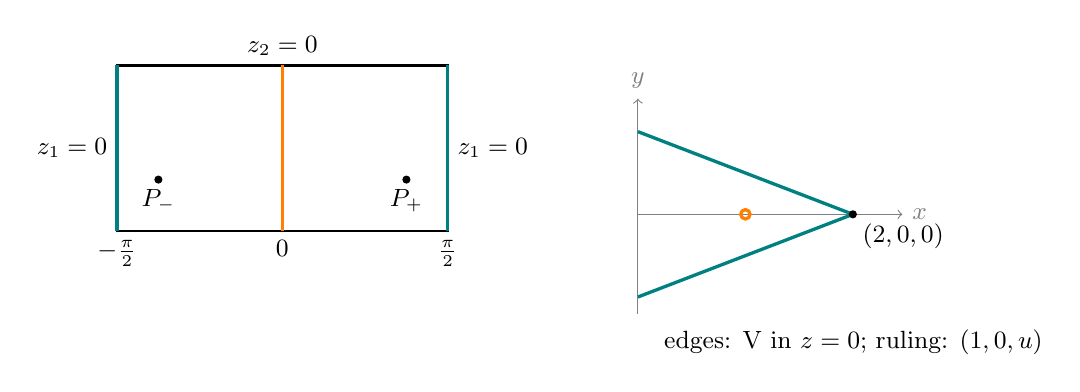
\begin{tikzpicture}[scale=1.05]
\draw[thick] (0,0) rectangle (4,2);
\draw[very thick,teal] (0,0)--(0,2); \draw[very thick,teal] (4,0)--(4,2);
\draw[very thick,orange] (2,0)--(2,2);
\node[below] at (0,0) {\small $-\frac\pi2$}; \node[below] at (2,0) {\small $0$};
\node[below] at (4,0) {\small $\frac\pi2$}; \node[left] at (0,1) {\small $z_1=0$};
\node[right] at (4,1) {\small $z_1=0$}; \node[above] at (2,2) {\small $z_2=0$};
\fill (0.50,0.62) circle (1.4pt) node[below] {\small $P_-$};
\fill (3.50,0.62) circle (1.4pt) node[below] {\small $P_+$};
\begin{scope}[xshift=6.3cm,yshift=0.2cm]
\draw[->,gray] (0,0)--(3.2,0) node[right]{\small $x$};
\draw[->,gray] (0,-1.2)--(0,1.4) node[above]{\small $y$};
\draw[very thick,teal] (0,1)--(2.6,0); \draw[very thick,teal] (0,-1)--(2.6,0);
\fill (2.6,0) circle (1.4pt) node[below right] {\small $(2,0,0)$};
\draw[very thick,orange] (1.3,0) circle (1.6pt);
\node[align=left,anchor=west] at (0.2,-1.55) {\small edges: V in $z=0$;\ ruling: $(1,0,u)$};
\end{scope}
\end{tikzpicture}
\caption{Ancestral powers vanish on the two edges ($z_1=0$) and on the polar
ruling ($z_2=0$). The edges map to a V in the plane $z=0$, which no analytic
image of $C_0$ can contain. The ruling (orange, vertical over $(1,0)$) maps to a
segment on a line skew to both legs.}\label{fig:edges}
\end{figure}

\begin{remark}[What extra data the historical model needs]\label{rem:data}
Theorem~\ref{thm:rigidity} gives a necessary edge criterion for any power
assignment $w=|z_1|^2$. Analytic readouts require $S(w^{-1}(0))$ to lie in the
image of an analytic loop, and phase-invariant readouts require it to be a
point. The same holds for $1-w$. The 0.02 assignment $(1-u,u)$ passes: its
vanishing edges $u=1$ and $u=0$ map to arcs of the circles $(x-1)^2+z^2=1$ and
$x^2+y^2=1$, and its quadratic readout maps the vanishing circles onto these
circles. The ancestral assignment fails, because $w^{-1}(0)$ consists of both edges.

Three additional inputs therefore remain, and none is supplied by the moment map.
One may use a non-analytic switching readout as in Theorem~\ref{thm:smooth}.
One may restrict to one half of the source, which loses a cross-cap and the
reflection pairing. Or one may change the powers, as continuation 0.02 does.
Approximation is cheap and carries no canonical content: by Weierstrass, real
polynomial readouts satisfy $\sup_D|P_\varepsilon\circ z-S|<\varepsilon$ for
every $\varepsilon>0$ with the family of Theorem~\ref{thm:smooth}, yet none is
exact. Whether a quadratic readout exists on $D_+$ is left open.
\end{remark}

\section{Exceptional pullback and folds of the observation map}\label{sec:shriek}
We work in the six-functor formalism on finite-dimensional locally compact
Hausdorff spaces with $D(X)=D(\mathrm{Sh}(X;\Z))$ \cite[Example 5.9]{scholze}.
Write $\omega_X=a_X^!\Z$ and $\mathbb D_X=\RHom(-,\omega_X)$. We use three
standard facts. First, Verdier duality gives $f^!\mathbb D_Y\simeq\mathbb D_Xf^*$
\cite[Prop.~4.6.9(3)]{knp}, \cite[Ch.~III]{ks}. Second, the stalk of $\omega_X$
at $x$ is local homology $H_*(X,X\setminus x)$, and $\omega_X\simeq\orr_X[n]$ for
an $n$-manifold without boundary \cite[Rem.~4.6.19, Cor.~4.6.20]{knp}. Third,
$f^!$ is local on the source, and open immersions satisfy $j^!=j^*$ and are
cohomologically smooth \cite[Rem.~5.4]{scholze}. Cohomological smoothness of
$f$ requires that $f^!\Z\otimes f^*(-)\to f^!(-)$ be an isomorphism, that
$f^!\Z$ be invertible, and that both survive base change \cite[Def.~5.1]{scholze}.
The draft's paraphrase ``$f^!\Z\simeq\Z[d]$'' records only the second condition.

\begin{theorem}[$f^!\Z$ sees only dimensions and boundary]\label{thm:shriek}
(1) For any continuous $f:X\to Y$ between topological manifolds without
boundary of dimensions $n$ and $m$,
$f^!\Z_Y\simeq\orr_X\otimes f^*\orr_Y[n-m]$.

(2) Let $D'\subset\R^2$ be a locally closed convex set with nonempty interior,
for instance $D$ or $D_\circ$, and let $j:\inte D'\to D'$ be the inclusion. For
every continuous $\Psi:D'\to\R^2$,
\[
 \Psi^!\Z_{\R^2}\simeq j_!\Z_{\inte D'}.
\]
Its stalk is $\Z$ in degree $0$ at interior points and $0$ at the remaining
points.
\end{theorem}
\begin{proof}
(1) Since $\omega_Y$ is invertible, $\Z_Y\simeq\mathbb D_Y\omega_Y$. Hence
\[
 f^!\Z_Y\simeq\mathbb D_Xf^*\omega_Y=\RHom(f^*\orr_Y[m],\orr_X[n]),
\]
and rank-one orientation systems are self-dual.

(2) For an interior point, $H_*(D',D'\setminus x)=\Z[2]$. For any other point
$x$, a point strictly between an interior point and a point of $D'$ is interior,
so $D'\setminus x$ is star-shaped about an interior point and hence
contractible. Local homology then vanishes. Thus $\omega_{D'}$ restricts to
$\Z[2]$ on the oriented interior and has zero stalks elsewhere. The counit
$j_!j^*\omega_{D'}\to\omega_{D'}$ is therefore a stalkwise isomorphism, and
$\omega_{D'}\simeq j_!\Z_{\inte D'}[2]$. Now
$\Psi^!\Z\simeq\mathbb D_{D'}\Psi^*\omega_{\R^2}=\RHom(\Z_{D'}[2],\omega_{D'})=\omega_{D'}[-2]$.
\end{proof}

\begin{corollary}[The draft shift]\label{cor:shift}
The observation map $\Psi=(N,M)$ of v7 Proposition~8.3 is defined and smooth on
$D_\circ$; since $M=P/Q$ and $Q=0$ at $t=\pm\pi/2$, it is not defined on all of $D$.
For every inclusion $i:L\to D_\circ$, $i^*\Psi^!\Z$ is $\Z$ on $L\cap\inte D_\circ$
and $0$ on the sides $u=0,1$.
The claimed $i^*\Psi^!\Z\simeq\Z[-1]$ on the fold locus holds at no point. The
``relative dimension'' is $0$ at every interior point, fold or not, contrary to
v7 Remark~8.16. If $L\subset\inte D_\circ$ is an embedded open arc, then
$i^!\Psi^!\Z\simeq\orr_L[-1]$. The shift $[-1]$ in the draft's local-cohomology sketch is the
codimension of $L$; it holds equally for arcs of regular points.
\end{corollary}
\begin{proof}
Restrict Theorem~\ref{thm:shriek}(2) with $D'=D_\circ$. For the arc,
$i^!\Z_{\inte D_\circ}=i^!\omega_{\inte D_\circ}[-2]=\omega_L[-2]=\orr_L[-1]$.
\end{proof}

The interior critical locus of $\Psi$ was determined in the published Stokes
paper \cite[Theorem~2.4]{stokes}. Every point of the symmetry segment with
$0<u<1$, and every interior point of the rational branch with $c_b<c<1$, is an
ordinary Whitney fold. At $(0,0)$ the ordinary-fold condition fails. The verifier
replays the Jacobian factorization and $N_{tt}(0,u)=-2u$.

\begin{proposition}[Where the fold is visible]\label{prop:detect}
Let $x\in\inte D_\circ$ be an ordinary fold point of $\Psi$. Choose disc
neighbourhoods $V\ni x$ and $W\ni\Psi(x)$ on which $f=\Psi|_V$ is
homeomorphic to $(\xi,\eta)\mapsto(\xi,\eta^2)$. Let $L$ be the fold arc and
$W'\subset W$ the open side of the discriminant containing $f(V\setminus L)$,
with inclusion $j'$. For $G=j'_!\Z_{W'}$:
\begin{enumerate}
\item $f^!\Z_W\simeq\Z_V$ is invertible and unshifted;
\item $f^*G\simeq(\Z_{V\setminus L})_!$ and $f^!G\simeq\Z_V$;
\item the comparison map $f^!\Z_W\otimes f^*G\to f^!G$ is injective with cokernel
$i_*\Z_L$; its stalks at $L$ are $0\to\Z$.
\end{enumerate}
Thus condition (1) of \cite[Def.~5.1]{scholze} fails at every ordinary fold
point, while condition (2) holds. At regular interior points $\Psi$ is a local
homeomorphism and is cohomologically smooth with $\Psi^!\Z\simeq\Z$.
\end{proposition}
\begin{proof}
(1) is Theorem~\ref{thm:shriek}(1). Pullback commutes with extension by zero,
and $f^{-1}(W')=V\setminus L$. Let $k:H\to W$ be the closed side
$\overline{W'}\cap W$. Its local homology vanishes on its edge, so
$\mathbb D_W(\Z_H)=k_*\omega_H\simeq G[2]$. Since $f(V)\subset H$,
\[
 f^!G[2]\simeq f^!\mathbb D_W(\Z_H)\simeq\mathbb D_V(f^*\Z_H)=\mathbb D_V\Z_V=\Z_V[2].
\]
Off $L$, $f$ is locally an open immersion, so the comparison map is an
isomorphism there. A morphism $(\Z_{V\setminus L})_!\to\Z_V$ is a locally
constant function on $V\setminus L$. Being invertible there, it takes values
$\pm1$. Its image is $(\Z_{V\setminus L})_!$, with cokernel $i_*\Z_L$.
\end{proof}

The fold is also seen by $f_*\Z_V$, whose stalk ranks are $2,1,0$ across the
discriminant, and on the surface side by the normalization defect sheaf already
proved in v12/v13. It is not seen by $f^!\Z$. Remark~8.4's appeal to Verdier
duality for the zero count is also unnecessary. The total index of the interior
zeros of $F=N+iM$ equals the winding number of $F$ along any loop in $D_\circ$
that encloses $P_\pm$ and avoids $(0,1)$. This is elementary degree theory.

\begin{proposition}[Carriers for the $\pm1$ sectors]\label{prop:carrier}
(1) Let $X$ be connected. Then $\End_{D(X)}(\Z_X)=H^0(X;\Z)=\Z$, every
involution of $\Z_X$ is $\pm\mathrm{id}$, and $\Z_X$ has no splitting into two
nonzero summands. Its characteristic polynomial is $t-1$ or $t+1$. For the constant
condensed sheaf on the compact connected image, the degree-zero endomorphisms
are again the continuous maps to $\Z$, so the conclusion is unchanged.

(2) Let $X=D_\circ\setminus\{P_+,P_-,(0,1)\}$, the set where $F\neq0$, and let
$\pi:\widetilde X\to X$ be the
double cover $\{\chi^2=F\}$. Then $\pi_*\Z$ is a rank-two local system with deck
involution $\tau$, and it is indecomposable over $\Z$. After inverting $2$,
$\pi_*\Z[\frac12]\simeq\Z[\frac12]_X\oplus\mathcal L[\frac12]$, where
$\mathcal L$ is the sign system with monodromy $-1$ around $P_+$ and around
$P_-$. In particular $\mathcal L$ does not extend over either point.

(3) A Whitney fold involution $(\xi,\eta)\mapsto(\xi,-\eta)$ fixes the fold arc
pointwise, whereas $\tau$ has no fixed points. Neither induces the other.
\end{proposition}
\begin{proof}
(1) Hom between sheaves in degree zero is $\Gamma(X,\mathcal Hom(\Z,\Z))$. For the
condensed constant sheaf on a compact Hausdorff space, global sections are
continuous maps to the discrete group $\Z$. Idempotents of $\Z$ are $0,1$.
(2) $N=0$ exactly on $c=1$ and on $u=(1-c)/2$. On the first, $M=1-u$; on the
second, $M$ is a positive multiple of $-(c^2-3c+1)$. Hence the zeros of $F$ in
$D_\circ$ are $(0,1)$ and $P_\pm$. The set $D_\circ\setminus\{(0,1)\}$ is
star-shaped about an interior point, so $\pi_1(X)$ is free on loops around $P_\pm$. The winding of $F$ is $\mp1$
there (Lean \texttt{actual\_dipole}; finite replay). Hence the monodromy of
$\pi$ is the surjection $\pi_1(X)\to C_2$, and the stalk of $\pi_*\Z$ is the
regular module $\Z[C_2]=\Z[x]/(x^2-1)$. Its only idempotents are $0$ and $1$
(verifier), so it is indecomposable. Over $\Z[\frac12]$ the projectors
$(1\pm x)/2$ split it.
(3) The fixed-point sets differ.
\end{proof}

Thus v7 Definition~8.9 to Corollary~8.11 place a rank-two $\pm1$ decomposition
on the rank-one constant sheaf, where (1) forbids it. The correct carrier of a
$-1$ sector is the sign system of the square-root cover, and it splits off
only after inverting $2$. The draft writes its projectors over $\Z[\frac12]$ but
its module over $\Z$. No map from the Mellin space $L^2([1,\infty))$ to either
carrier is supplied, so the claimed inclusion of the Mellin domain in the
$+1$ sector has no object to refer to.

\section{Log-scale versus linear-scale windows}\label{sec:windows}
Let $K(\delta,L)=L^{-1}\int_0^Le^{-i\delta\tau}d\tau$ for real $\delta\neq0$. Then
$|K(\delta,L)|=|\sin(\delta L/2)|/(|\delta|L/2)\leq2/(|\delta|L)$.

\begin{proposition}[Window masses, not arithmetic]\label{prop:windows}
Let $T>1$.
\begin{enumerate}
\item $\frac1{\log T}\int_1^Tx^{-i\delta}\frac{dx}x=K(\delta,\log T)$ and
$\frac1T\int_0^Te^{-i\delta t}dt=K(\delta,T)$. The two v7 bounds are one bound,
$2/(|\delta|\cdot\text{window mass})$, evaluated at masses $\log T$ and $T$.
Their ratio $T/\log T$ is the same for every real $\delta$, whether or not
$\delta=\log(n/m)$. The exact ratio of the moduli is
$(T/\log T)\,|\sin(\delta\log T/2)/\sin(\delta T/2)|$. Along
$T_k=(2k+1)\pi/|\delta|$ the second factor equals $|\sin(\delta\log T_k/2)|$,
whose $\liminf$ is $0$ and $\limsup$ is $1$.
\item For the same characters $x^{-i\delta}$ on the same interval $[1,T]$ with
Lebesgue measure,
\[
 \frac1{T-1}\int_1^Tx^{-i\delta}dx=\frac{T^{1-i\delta}-1}{(1-i\delta)(T-1)},
\]
whose modulus tends to $(1+\delta^2)^{-1/2}\neq0$. There is no decorrelation at
all; with Haar measure the decay is $O(1/\log T)$. The ordering claimed by
Remark~8.14 is reversed.
\item For the time phasors $e^{-i\delta t}$ on $[1,T]$ with Haar measure,
$\bigl|\frac1{\log T}\int_1^Te^{-i\delta t}\frac{dt}t\bigr|\leq\frac2{|\delta|\log T}$.
\end{enumerate}
\end{proposition}
\begin{proof}
(1) Substitute $x=e^\tau$. Along $T_k$, $\delta\log T_k/2$ tends to infinity
with increments tending to zero, so it comes arbitrarily close to every residue
modulo $\pi$. (2) Integrate directly. (3) Integrate by parts once; the boundary
terms and the remaining integral contribute at most $2/|\delta|$ in total.
\end{proof}

In no reading does integrality enter. Moreover $\mathbb N$ is not a subgroup
of $(\R_{>0},\times)$; the subgroup it generates is $\Q_{>0}$, which is dense.
The proposed aliasing and Weil-group interpretation of Remark~8.14 therefore
has no quantity to explain.

\section{Status and open questions}\label{sec:status}
\begin{center}\small
\begin{tabular}{>{\raggedright\arraybackslash}p{.24\linewidth}>{\raggedright\arraybackslash}p{.44\linewidth}>{\raggedright\arraybackslash}p{.22\linewidth}}\toprule
Historical item & Result here & Evidence\\\midrule
Moment derivation of $S$ (v7/ancestor/v12 \S3, Def.~3.1) & Phase-invariant, mixed-state and analytic readouts excluded; $C^\infty$ realization exists; one half admits analytic but not affine readouts & Written proofs; exact/finite replay\\
v7 Prop.~8.3, Rem.~8.16 & $\Psi^!\Z\simeq j_!\Z_{\inte D'}$ for every continuous $\Psi$ on a convex $D'$; draft shift false; fold detected by the comparison map & Written proofs from cited duality theorems\\
v7 Def.~8.9--Cor.~8.11 & $\End(\Z_X)=\Z$; correct carrier is the indecomposable $\pi_*\Z$, split only over $\Z[\frac12]$ & Written proof; winding and idempotent replay\\
v7 Prop.~8.13, Rem.~8.14 & Gap is the window-mass ratio; same characters with Lebesgue measure do not decorrelate & Exact integrals; finite replay\\\bottomrule
\end{tabular}
\end{center}

Nothing in this note is Lean-formalized; the own Lean inventory stays at 33
theorems. The external inputs are the Verdier-duality facts cited above and the
Stokes fold classification. Open questions include a quadratic readout on
$D_+$; a canonical choice among non-analytic historical readouts, which
Theorem~\ref{thm:smooth} suggests does not exist without further principles; and
a genuinely sign-twisted analytic carrier compatible with the actual Green and
Dirac operators. The actual singular Dirac and Pin problems of v12 \S8.20--8.24
are untouched here.

{\small\begin{thebibliography}{9}
\bibitem{scholze} P. Scholze, \emph{Six-Functor Formalisms}, lecture notes,
 arXiv:2510.26269v2 (22 January 2026), Definition~5.1 and Remark~5.4 (p.~32),
 Example~5.9 (p.~36). \url{https://arxiv.org/abs/2510.26269}.
\bibitem{knp} A. Krause, T. Nikolaus and P. P\"utzst\"uck, \emph{Sheaves on
 Manifolds}, lecture notes, 7 November 2024, \S4.6, Proposition~4.6.9,
 Remark~4.6.19, Corollary~4.6.20; Theorem~1.1.10.
\bibitem{ks} M. Kashiwara and P. Schapira, \emph{Sheaves on Manifolds},
 Grundlehren 292, Springer, 1990, Chapter III. Standard reference; not
 retrieved in this round.
\bibitem{stokes} A. Hayami (J.-Y. Huang), \emph{Observation Discriminant and
 Spherical Fold Image of the Orthogonal-Circle Ruled Surface} (Stokes v5),
 Zenodo, DOI \href{https://doi.org/10.5281/zenodo.22728902}{10.5281/zenodo.22728902};
 Theorem~2.4 (``Ordinary folds and the exceptional intersection'') of the
 registered final PDF.
\end{thebibliography}}
\end{document}
